% move all configuration stuff into includes file so we can focus on the content
\documentclass[aspectratio=169,hyperref={pdfpagelabels=false,colorlinks=true,linkcolor=white,urlcolor=blue},t]{beamer}

%%%%%%%%%%%%%%%%%%%%%%%%%%%%%%%%%%%%%%%%%%%%%%%%%%%%%%%%%%%%%%%%%%%%%%%%%%%%%%%%%%
%%%%%%%%%%%%%%%%%%%%%%%%%%%%%%%%%%%%%%%%%%%%%%%%%%%%%%%%%%%%%%%%%%%%%%%%%%%%%%%%%%
% packages
\usepackage{pict2e}
\usepackage{epic}
\usepackage{amsmath,amsfonts,amssymb}
\usepackage{units}
\usepackage{fancybox}
\usepackage[absolute,overlay]{textpos} 
\usepackage{media9} % avi2flv: "C:\Program Files\ffmpeg\bin\ffmpeg.exe" -i TuneFreqFilterbank.avi -b 600k -s 441x324 -r 15 -acodec copy TuneFreqFilterbank.flv
\usepackage{animate}
\usepackage{gensymb}
\usepackage{multirow}
\usepackage{silence}
\usepackage{tikz}
\usepackage[backend=bibtex,style=ieee]{biblatex}
\AtEveryCitekey{\iffootnote{\tiny}{}}
\addbibresource{include/references}

%%%%%%%%%%%%%%%%%%%%%%%%%%%%%%%%%%%%%%%%%%%%%%%%%%%%%%%%%%%%%%%%%%%%%%%%%%%%%%%%%%
%%%%%%%%%%%%%%%%%%%%%%%%%%%%%%%%%%%%%%%%%%%%%%%%%%%%%%%%%%%%%%%%%%%%%%%%%%%%%%%%%%
% relative paths
\graphicspath{{graph/}}


%%%%%%%%%%%%%%%%%%%%%%%%%%%%%%%%%%%%%%%%%%%%%%%%%%%%%%%%%%%%%%%%%%%%%%%%%%%%%%%%%%
%%%%%%%%%%%%%%%%%%%%%%%%%%%%%%%%%%%%%%%%%%%%%%%%%%%%%%%%%%%%%%%%%%%%%%%%%%%%%%%%%%
% units
\setlength{\unitlength}{1mm}

%%%%%%%%%%%%%%%%%%%%%%%%%%%%%%%%%%%%%%%%%%%%%%%%%%%%%%%%%%%%%%%%%%%%%%%%%%%%%%%%%%
%%%%%%%%%%%%%%%%%%%%%%%%%%%%%%%%%%%%%%%%%%%%%%%%%%%%%%%%%%%%%%%%%%%%%%%%%%%%%%%%%%
% theme & layout
\usetheme{Frankfurt}
\beamertemplatenavigationsymbolsempty
%\setbeamertemplate{frametitle}[smoothbars theme]
\setbeamertemplate{frametitle}
{
    \begin{beamercolorbox}[ht=1.8em,wd=\paperwidth]{frametitle}
        \vspace{-.1em}%
        \hspace{.2em}{\strut\insertframetitle\strut}
        
        \hspace{.2em}\small\strut\insertframesubtitle\strut
        %\hfill
        %\includegraphics[height=.8cm,keepaspectratio]{CenterMusicTechnology-solid-2lines-white-CoAtag}
        
    \end{beamercolorbox}
    \begin{textblock*}{100mm}(11.6cm,.7cm)
        \includegraphics[height=.8cm,keepaspectratio]{Logo_GTCMT_black}
    \end{textblock*}
}
\setbeamertemplate{footline}[frame number]

% set this to ensure bulletpoints without subsections
\usepackage{remreset}
\makeatletter
\@removefromreset{subsection}{section}
\makeatother
\setcounter{subsection}{1}

%---------------------------------------------------------------------------------
% appearance
\setbeamercolor{structure}{fg=gtgold}
\setbeamercovered{transparent} %invisible
\setbeamercolor{bibliography entry author}{fg=black}
\setbeamercolor*{bibliography entry title}{fg=black}
\setbeamercolor*{bibliography entry note}{fg=black}
\setbeamercolor{frametitle}{fg=black}
\setbeamercolor{title}{fg=black}

%\usepackage{pgfpages}
%\setbeameroption{show notes}
%\setbeameroption{show notes on second screen=right}
%---------------------------------------------------------------------------------
% fontsize
\let\Tiny=\tiny

%%%%%%%%%%%%%%%%%%%%%%%%%%%%%%%%%%%%%%%%%%%%%%%%%%%%%%%%%%%%%%%%%%%%%%%%%%%%%%%%%%
%%%%%%%%%%%%%%%%%%%%%%%%%%%%%%%%%%%%%%%%%%%%%%%%%%%%%%%%%%%%%%%%%%%%%%%%%%%%%%%%%%
% warnings
\pdfsuppresswarningpagegroup=1
\WarningFilter{biblatex}{Patching footnotes failed}
\WarningFilter{latexfont}{Font shape}
\WarningFilter{latexfont}{Some font shapes}
\WarningFilter{gensymb}{Not defining}


%%%%%%%%%%%%%%%%%%%%%%%%%%%%%%%%%%%%%%%%%%%%%%%%%%%%%%%%%%%%%%%%%%%%%%%%%%%%%%%%%%
%%%%%%%%%%%%%%%%%%%%%%%%%%%%%%%%%%%%%%%%%%%%%%%%%%%%%%%%%%%%%%%%%%%%%%%%%%%%%%%%%%
% theme & layout
\usetheme{Frankfurt}
\useinnertheme{rectangles}


%%%%%%%%%%%%%%%%%%%%%%%%%%%%%%%%%%%%%%%%%%%%%%%%%%%%%%%%%%%%%%%%%%%%%%%%%%%%%%%%%%
\setbeamertemplate{frametitle}[default][colsep=-4bp,rounded=false,shadow=false]
\setbeamertemplate{frametitle}
{%
    \nointerlineskip%
    %\vskip-0.5ex
    \begin{beamercolorbox}[wd=\paperwidth,ht=3.5ex,dp=0.6ex]{frametitle}
        \hspace*{1.3ex}\insertframetitle%
        
        \hspace*{1.3ex}\small\insertframesubtitle%
    \end{beamercolorbox}%
    \begin{textblock*}{100mm}(11.6cm,.57cm)
        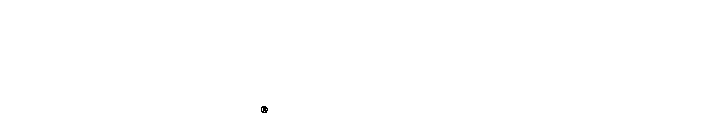
\includegraphics[height=.8cm,keepaspectratio]{graph/Logo_GTCMT_white}
    \end{textblock*}
}


%%%%%%%%%%%%%%%%%%%%%%%%%%%%%%%%%%%%%%%%%%%%%%%%%%%%%%%%%%%%%%%%%%%%%%%%%%%%%%%%%%
\setbeamertemplate{title page}[default][colsep=-4bp,rounded=false,shadow=false]
\setbeamertemplate{title page}
{
    \begin{textblock*}{100mm}(15cm,.51cm)
            \href{https://github.com/alexanderlerch/ACA-Slides/blob/2nd_edition/\jobname.pdf}{\includegraphics[height=.5cm,keepaspectratio]{graph/Logo_github}}\hspace*{2ex}
    \end{textblock*}
    \vskip-10ex
    \begin{beamercolorbox}[wd=\paperwidth,ht=.7\paperheight,dp=0.6ex]{frametitle} %35ex
        %\begin{flushright}
            %\href{http://www.gtcmt.gatech.edu}{\includegraphics[height=.8cm,keepaspectratio]{graph/Logo_GTCMT_black}}\hspace*{2ex}
        %\end{flushright}
        
        \hspace*{1.8ex}\LARGE\inserttitle%
        
        \vspace*{.5ex}
        
        \hspace*{1.3ex}\small\insertsubtitle%
        
        \vspace*{.5ex}
    \end{beamercolorbox}%
    \nointerlineskip%
    \begin{beamercolorbox}[wd=\paperwidth,ht=.4\paperheight,dp=0.6ex]{page number in head/foot}
        %\vspace*{-.5ex}
        \hspace*{1.7ex}\small\insertauthor%
        
        %\hspace*{1.7ex}\small }%
        
        \vspace*{10ex}
        
        \begin{flushright}
            \href{http://www.gtcmt.gatech.edu}{\includegraphics[height=.8cm,keepaspectratio]{graph/Logo_GTCMT_black}}\hspace*{2ex}
        \end{flushright}
    \end{beamercolorbox}%
}


%%%%%%%%%%%%%%%%%%%%%%%%%%%%%%%%%%%%%%%%%%%%%%%%%%%%%%%%%%%%%%%%%%%%%%%%%%%%%%%%%%
%\makeatother
\setbeamertemplate{footline}
{
  \leavevmode%
  \hbox{%
  \begin{beamercolorbox}[wd=.5\paperwidth,ht=2.25ex,dp=1ex,left,leftskip=1ex]{page number in head/foot}%
    \insertsubtitle
  \end{beamercolorbox}%
  \begin{beamercolorbox}[wd=.5\paperwidth,ht=2.25ex,dp=1ex,right,rightskip=1ex]{page number in head/foot}%
    \hfill
    \insertframenumber{} / \inserttotalframenumber
  \end{beamercolorbox}}%
  \vskip0pt%
}
%\makeatletter


%%%%%%%%%%%%%%%%%%%%%%%%%%%%%%%%%%%%%%%%%%%%%%%%%%%%%%%%%%%%%%%%%%%%%%%%%%%%%%%%%%
\beamertemplatenavigationsymbolsempty
\setbeamertemplate{navigation symbols}{}
\setbeamertemplate{blocks}[default]%[rounded=false,shadow=false]
\setbeamertemplate{itemize item}[square]
\setbeamertemplate{itemize subitem}[circle]
\setbeamertemplate{itemize subsubitem}[triangle]
\setbeamertemplate{enumerate item}[square]
\setbeamertemplate{enumerate subitem}[circle]
\setbeamertemplate{enumerate subsubitem}[circle]


%%%%%%%%%%%%%%%%%%%%%%%%%%%%%%%%%%%%%%%%%%%%%%%%%%%%%%%%%%%%%%%%%%%%%%%%%%%%%%%%%%
% colors
\setbeamercolor{structure}{fg=darkgray}
\setbeamercovered{transparent} %invisible
\setbeamercolor{bibliography entry author}{fg=black}
\setbeamercolor*{bibliography entry title}{fg=black}
\setbeamercolor*{bibliography entry note}{fg=black}
\setbeamercolor{frametitle}{fg=black}
\setbeamercolor{title}{fg=white}
\setbeamercolor{subtitle}{fg=white}
\setbeamercolor{frametitle}{fg=white}
\setbeamercolor{framesubtitle}{fg=white}
\setbeamercolor{mini frame}{fg=white, bg=black}
\setbeamercolor{section in head/foot}{fg=white, bg=darkgray}
\setbeamercolor{page number in head/foot}{fg=black, bg=lightblue}
\setbeamercolor{item projected}{fg=white, bg=black}

%---------------------------------------------------------------------------------
%%%%%%%%%%%%%%%%%%%%%%%%%%%%%%%%%%%%%%%%%%%%%%%%%%%%%%%%%%%%%%%%%%%%%%%%%%%%%%%%%%
%%%%%%%%%%%%%%%%%%%%%%%%%%%%%%%%%%%%%%%%%%%%%%%%%%%%%%%%%%%%%%%%%%%%%%%%%%%%%%%%%%
% title information
\title[]{Introduction to \textbf{Audio Content Analysis}}   
\author[alexander lerch]{alexander lerch} 
%\institute{~}
%\date[Alexander Lerch]{}
%\titlegraphic{\vspace{-16mm}\includegraphics[width=\textwidth,height=3cm]{title}}

%%%%%%%%%%%%%%%%%%%%%%%%%%%%%%%%%%%%%%%%%%%%%%%%%%%%%%%%%%%%%%%%%%%%%%%%%%%%%%%%%%
%%%%%%%%%%%%%%%%%%%%%%%%%%%%%%%%%%%%%%%%%%%%%%%%%%%%%%%%%%%%%%%%%%%%%%%%%%%%%%%%%%
% colors
\definecolor{gtgold}{HTML}{E0AA0F} %{rgb}{0.88,0.66,1,0.06} [234, 170, 0]/256
\definecolor{darkgray}{rgb}{.1, .1, .25}
\definecolor{lightblue}{rgb}{.1, 0.75, 1}
\definecolor{highlight}{rgb}{0, 0, 1} %_less!40

%%%%%%%%%%%%%%%%%%%%%%%%%%%%%%%%%%%%%%%%%%%%%%%%%%%%%%%%%%%%%%%%%%%%%%%%%%%%%%%%%%
%%%%%%%%%%%%%%%%%%%%%%%%%%%%%%%%%%%%%%%%%%%%%%%%%%%%%%%%%%%%%%%%%%%%%%%%%%%%%%%%%%
% relative paths
\graphicspath{{../ACA-Plots/graph/}}


%%%%%%%%%%%%%%%%%%%%%%%%%%%%%%%%%%%%%%%%%%%%%%%%%%%%%%%%%%%%%%%%%%%%%%%%%%%%%%%%%%
%%%%%%%%%%%%%%%%%%%%%%%%%%%%%%%%%%%%%%%%%%%%%%%%%%%%%%%%%%%%%%%%%%%%%%%%%%%%%%%%%%
% units
\setlength{\unitlength}{1mm}

%%%%%%%%%%%%%%%%%%%%%%%%%%%%%%%%%%%%%%%%%%%%%%%%%%%%%%%%%%%%%%%%%%%%%%%%%%%%%%%%%%
%%%%%%%%%%%%%%%%%%%%%%%%%%%%%%%%%%%%%%%%%%%%%%%%%%%%%%%%%%%%%%%%%%%%%%%%%%%%%%%%%%
% math
\DeclareMathOperator*{\argmax}{argmax}
\DeclareMathOperator*{\argmin}{argmin}
\DeclareMathOperator*{\atan}{atan}
\DeclareMathOperator*{\arcsinh}{arcsinh}
\DeclareMathOperator*{\sign}{sign}
\DeclareMathOperator*{\tcdf}{tcdf}
\DeclareMathOperator*{\si}{sinc}
\DeclareMathOperator*{\princarg}{princarg}
\DeclareMathOperator*{\arccosh}{arccosh}
\DeclareMathOperator*{\hwr}{HWR}
\DeclareMathOperator*{\flip}{flip}
\DeclareMathOperator*{\sinc}{sinc}
\DeclareMathOperator*{\floor}{floor}
\newcommand{\e}{{e}}
\newcommand{\jom}{\mathrm{j}\omega}
\newcommand{\jOm}{\mathrm{j}\Omega}
\newcommand   {\mat}[1]    		{\boldsymbol{\uppercase{#1}}}		%bold
\renewcommand {\vec}[1]    		{\boldsymbol{\lowercase{#1}}}		%bold

%%%%%%%%%%%%%%%%%%%%%%%%%%%%%%%%%%%%%%%%%%%%%%%%%%%%%%%%%%%%%%%%%%%%%%%%%%%%%%%%%%
%%%%%%%%%%%%%%%%%%%%%%%%%%%%%%%%%%%%%%%%%%%%%%%%%%%%%%%%%%%%%%%%%%%%%%%%%%%%%%%%%%
% media9
\newcommand{\includeaudio}[1]{
\href{run:audio/#1.mp3}{
\includegraphics[width=5mm, height=5mm]{graph/SpeakerIcon}}}

\newcommand{\includeanimation}[4]{{\begin{center}
                        \animategraphics[autoplay,loop,scale=.7]{#4}{animation/#1-}{#2}{#3}        
                        \end{center}
                        \addreference{matlab source: \href{https://github.com/alexanderlerch/ACA-Plots/blob/master/matlab/animate#1.m}{matlab/animate#1.m}}}
                        \inserticon{video}}
                        
%%%%%%%%%%%%%%%%%%%%%%%%%%%%%%%%%%%%%%%%%%%%%%%%%%%%%%%%%%%%%%%%%%%%%%%%%%%%%%%%%%
%%%%%%%%%%%%%%%%%%%%%%%%%%%%%%%%%%%%%%%%%%%%%%%%%%%%%%%%%%%%%%%%%%%%%%%%%%%%%%%%%%
% other commands
\newcommand{\question}[1]{%\vspace{-4mm}
                          \setbeamercovered{invisible}
                          \begin{columns}[T]
                            \column{.9\textwidth}
                                \textbf{#1}
                            \column{.1\textwidth}
                                \vspace{-8mm}
                                \begin{flushright}
                                     
\includegraphics[width=.9\columnwidth]{graph/question_mark}
                                \end{flushright}
                                \vspace{6mm}
                          \end{columns}\pause\vspace{-12mm}}

\newcommand{\toremember}[1]{
                        \inserticon{lightbulb}
                        }

\newcommand{\matlabexercise}[1]{%\vspace{-4mm}
                          \setbeamercovered{invisible}
                          \begin{columns}[T]
                            \column{.8\textwidth}
                                \textbf{matlab exercise}: #1
                            \column{.2\textwidth}
                                \begin{flushright}
                                     \includegraphics[scale=.5]{graph/logo_matlab}
                                \end{flushright}
                                %\vspace{6mm}
                          \end{columns}}

\newcommand{\addreference}[1]{  
                  
                    \begin{textblock*}{\baselineskip }(.98\paperwidth,.5\textheight) %(1.15\textwidth,.4\textheight)
                         \begin{minipage}[b][.5\paperheight][b]{1cm}%
                            \vfill%
                             \rotatebox{90}{\tiny {#1}}
                        \end{minipage}
                   \end{textblock*}
                    }
                    
\newcommand{\figwithmatlab}[1]{
                    \begin{figure}
                        \centering
                        \includegraphics[scale=.7]{#1}
                        %\label{fig:#1}
                    \end{figure}
                    
                    \addreference{matlab source: \href{https://github.com/alexanderlerch/ACA-Plots/blob/main/matlab/plot#1.m}{plot#1.m}}}
\newcommand{\figwithref}[2]{
                    \begin{figure}
                        \centering
                        \includegraphics[scale=.7]{#1}
                        \label{fig:#1}
                    \end{figure}
                    
                    \addreference{#2}}  
                                    
\newcommand{\inserticon}[1]{
                    \begin{textblock*}{100mm}(14.5cm,7.5cm)
                        \includegraphics[height=.8cm,keepaspectratio]{graph/#1}
                    \end{textblock*}}            

%%%%%%%%%%%%%%%%%%%%%%%%%%%%%%%%%%%%%%%%%%%%%%%%%%%%%%%%%%%%%%%%%%%%%%%%%%%%%%%%%%
%%%%%%%%%%%%%%%%%%%%%%%%%%%%%%%%%%%%%%%%%%%%%%%%%%%%%%%%%%%%%%%%%%%%%%%%%%%%%%%%%%
% counters
\newcounter{i}
\newcounter{j}
\newcounter{iXOffset}
\newcounter{iYOffset}
\newcounter{iXBlockSize}
\newcounter{iYBlockSize}
\newcounter{iYBlockSizeDiv2}
\newcounter{iXBlockSizeDiv2}
\newcounter{iDistance}



\subtitle{module 3.7.4: feature dimensionality reduction}

%%%%%%%%%%%%%%%%%%%%%%%%%%%%%%%%%%%%%%%%%%%%%%%%%%%%%%%%%%%%%%%%%%%%%%%%%%%%
\begin{document}
    % generate title page
	{
\setbeamertemplate{headline}{} 
\setbeamertemplate{footline}{} 
\begin{frame}
    \titlepage
    %\vspace{-5mm}
\end{frame}
}
\addtocounter{framenumber}{-1}


    \section[overview]{lecture overview}
        \begin{frame}{introduction}{overview}
            \begin{block}{corresponding textbook section}
                    %\href{http://ieeexplore.ieee.org/xpl/articleDetails.jsp?arnumber=6331120}{Chapter 3~---~Instantaneous Features}: pp.~63--66
                    section~3.7.4\\
                    appendix~C
            \end{block}

            \begin{itemize}
                \item   \textbf{lecture content}
                    \begin{itemize}
                        \item   problems of dimensionality
                        \item   feature selection
                        \item   feature transformation/mapping
                    \end{itemize}
                \bigskip
                \item<2->   \textbf{learning objectives}
                    \begin{itemize}
                        \item   describe potential challenges with high-dimensional feature spaces
                        \item   discuss advantages and disadvantages of various methods for feature selection
                        \item   summarize PCA as feature transformation method
                    \end{itemize}
            \end{itemize}
            \inserticon{directions}
        \end{frame}

   \section[intro]{introduction}
		\begin{frame}{introduction}{dimensionality reduction}
            \begin{itemize}
                \item   \textbf{problem}
                    \begin{itemize}
                        \item   many ML approaches cannot cope with large amounts of irrelevant features
                        \item   ML algorithms might degrade in performance
                    \end{itemize}
                \bigskip
                \item<2->   \textbf{advantages}
                    \begin{itemize}
                        \item   reducing storage requirements
                        \item   reducing training complexity
                        \item   defying the ``curse of dimensionality''
                    \end{itemize}
                \bigskip
                \item<3->   \textbf{disadvantages}
                    \begin{itemize}
                        \item   additional workload for reduction
                        \item   adding an additional layer of model complexity
                    \end{itemize}
            \end{itemize}
		\end{frame}
        
		\begin{frame}{introduction}{dimensionality issues}
            \vspace{-2mm}
            problems of high-dimensional data:
            \begin{itemize}
                \item   increase in run-time
                \item   overfitting
                \item   curse of dimensionality
                \item   required amount of training samples 
            \end{itemize}
			
			\only<2->{
            \smallskip
			$\Rightarrow$ increasing number of input features may \textit{decrease} classification performance
            \figwithmatlab{SequentialForwardSelection}
            }
		\end{frame}

    \section[challenges]{high data dimensionality challenges}
		\begin{frame}{dimensionality issues}{overfitting}
            \vspace{-5mm}
            \begin{columns}
            \column{.4\linewidth}
            \begin{itemize}
                \item   \textbf{overfitting}:
                    \begin{itemize}
                        \item   lack of training data
                        \item   overly complex model
                        \item[$\Rightarrow$]<2-> model cannot be estimated properly
                    \end{itemize}
                    
                    \bigskip
                    \item<2-> required training set size depends on 
                        \begin{itemize}
                            \item   classifier (parametrization)
                            \item   number of classes
                            \item   task complexity
                            \bigskip
                            \item[$\Rightarrow$]<3-> \textit{rule of thumb}:\\ don't bother with training sets smaller than $\mathcal{F}^2$
                        \end{itemize}
                    
			\end{itemize}
            \column{.6\linewidth}
                    \figwithmatlab{Overfitting}
            \end{columns}
		\end{frame}
		\begin{frame}{dimensionality issues}{curse of dimensionality}
            \only<1>{
            \begin{itemize}
                \item \textbf{curse of dimensionality}: 
                    \begin{itemize}
                        \item   increasing dimensionality leads to sparse training data
                        \item   neighborhoods of data points become less concentrated
                        \item   model tends to be harder to estimate in higher-dimensional space
                        \item   applies to distance-based algorithms
                    \end{itemize}
            \end{itemize}
            }
            \only<2->{
             \textbf{example} (uniformly distributed data): identify region on axis covering \textbf{1\% of data}
            \begin{columns}
            \column{.3\linewidth}
            %\begin{itemize}
                %\item  
                    %\begin{itemize}
                        %\item   
                            \begin{itemize}
                                \item   1-D: 1\% of x-axis
                                \item   2-D: 10\% of x/y-axis
                                \item   3-D: 21.5\% of x/y/z-axis
                                \item   10-D: 63\%
                                \item   100-D: 95\%
                            \end{itemize}
                    %\end{itemize}
            %\end{itemize}
            \column{.7\linewidth}
            \includeanimation{CurseOfDimensionality}{00}{02}{1}
            %\vspace{-8mm}
            %\begin{center}
                %\animategraphics[loop]{1}{-}{00}{02}        
            %\end{center}
            \end{columns}
            }
		\end{frame}

    \section[reduction]{dimensionality reduction}
		\begin{frame}{dimensionality reduction}{introduction}
			\begin{itemize}
				\item	\textbf{feature subset selection}:\\ discard least helpful features
                    \pause
                    \begin{itemize}
                        \item	high ``discriminative'' or descriptive power
                        \item	non-correlation to other features
                        \item	invariance to irrelevancies
                    \end{itemize}
				\bigskip
				\item<2->	\textbf{feature space transformation}:\\ map feature space
			\end{itemize}
		\end{frame}
        
    \section[selection]{feature subset selection}
		\begin{frame}{feature subset selection}{manual feature selection}
            \begin{columns}[T]
            \column{.2\linewidth}
                example scatter plots of pairs of features in a multi-class scenario
            \column{.8\linewidth}
                \figwithmatlab{FeatureScatter}
%                \begin{figure}
%                    \centering
%                    \hspace{-5mm}\vspace{-5mm}
                    %\includegraphics{noise_subfeatures}
%                \end{figure}
            \end{columns}
		\end{frame}
        
		\begin{frame}{feature subset selection}{introduction}
            \vspace{-3mm}
			\begin{enumerate}
				\item	\textbf{wrapper methods}:
                    \begin{itemize}
                        \item \textit{description}
                            \begin{itemize}
                                \item  use the ``classifier'' itself to evaluate feature performance
                            \end{itemize}
                         \item \textit{advantages}
                            \begin{itemize}
                                \item   taking into account feature dependencies
                                \item   model dependency
                            \end{itemize}
                         \item \textit{disadvantages}
                            \begin{itemize}
                                \item   complexity
                                \item   risk of overfitting
                            \end{itemize}
                  \end{itemize}
				
				\smallskip
                \item<2->	\textbf{filter methods}:
                    \begin{itemize}
                        \item \textit{description}
                            \begin{itemize}
                                \item  use an objective function
                            \end{itemize}
                         \item<2-> \textit{advantages}
                            \begin{itemize}
                                \item   easily scalable
                                \item   independent of classification algorithm
                            \end{itemize}
                         \item<2-> \textit{disadvantages}
                            \begin{itemize}
                                \item   no interaction with classifier
                                \item   no feature dependencies
                            \end{itemize}
                    \end{itemize}
			\end{enumerate}
		\end{frame}

        %\begin{frame}{excursion}{simple classifier~---~nearest neighbor}
            %\vspace{-3mm}
            %\begin{itemize}
                %\item	    \textbf{training}:
                    %\begin{itemize}
                        %\item store feature vector (\& class label) of each training sample
                    %\end{itemize}
                %\item<2->	\textbf{classification}:
                    %\begin{itemize}
                        %\item for new file/feature vector, detect \textit{closest training point}
                        %\item   choose closest point's class as result
                    %\end{itemize}
            %\end{itemize}
            %\vspace{-4mm}
            %\only<1>{
                %\figwithmatlab{Scatter}
            %}
            %\only<2->{
                %\figwithref{Scatter-nn}{matlab source: matlab/displayScatter.m}
            %}
        %\end{frame}
        
		\begin{frame}{feature subset selection}{wrapper methods 1/2}
            \vspace{-2mm}
			\begin{enumerate}
				\item	\textbf{single variable classification}:
                    \begin{itemize}
                        \item   \textit{procedure}
                            \begin{itemize}
                                \item   evaluate each feature individually
                                \item   choose the top $N$
                            \end{itemize}
                        \item<1->  \textit{complexity} 
                            \begin{itemize}
                                \item   subsets to test: $\mathcal{F}$
                            \end{itemize}
                        \item<1->   \textit{challenges}
                            \begin{itemize}
                                \item	inter-feature correlation is not considered
                                \item	feature combinations are not considered
                            \end{itemize}
                    \end{itemize}
				\smallskip 
                \item<2->	\textbf{brute force subset selection}
                    \begin{itemize}
                        \item   \textit{procedure}
                            \begin{itemize}
                                \item   evaluate all possible feature combinations
                                \item   choose the optimal combination
                            \end{itemize}
                        \item<2->  \textit{complexity} 
                            \begin{itemize}
                                \item   subsets to test: $2^\mathcal{F}$
                            \end{itemize}
                    \end{itemize}
			\end{enumerate}
		\end{frame}
		\begin{frame}{feature subset selection}{wrapper methods 2/2}
            \vspace{-2mm}
			\begin{enumerate}
                \setcounter{enumi}{3}
				\item	\textbf{sequential forward selection}
                    \begin{itemize}
                        \item   \textit{procedure}
                            \begin{enumerate}
                                \item	init: empty feature subset $\mathcal{V}_\mathrm{s} = {\emptyset}$
                                \item<1->	find feature $v_j$ maximizing objective function
                                            \begin{equation*}
                                                v_j = \argmax_{\forall j | v_j \notin \mathcal{V}_\mathrm{s}} J({\mathcal{V}_\mathrm{s}} \bigcup v_j) 
                                            \end{equation*}
                                \item<1->	add feature $v_j$ to $\mathcal{V}_\mathrm{s}$ 
                                \item<1->	go to step $2$
                            \end{enumerate}
                    \end{itemize}
					
				\smallskip
                \item<2->	\textbf{sequential backward elimination}
                    \begin{itemize}
                        \item   \textit{procedure}
                            \begin{enumerate}
                                \item	init: full feature set
                                \item<2->	find feature $v_j$ with the least impact on objective function
                                \item<2->	discard feature $v_j$
                                \item<2->	go to step $2$
                            \end{enumerate}
                    \end{itemize}
			\end{enumerate}
		\end{frame}
        
    \section[mapping]{feature space transformation}
		\begin{frame}{feature space transformation}{PCA introduction}
            \begin{itemize}
                \item   \textbf{objective}
                    \begin{itemize}
                        \item   map features to new coordinate system
                            \begin{equation*}\label{eq:pca_an}
                                \vec{u}(n) = \mat{T}^\mathrm{T}\cdot\vec{v}(n) 
                            \end{equation*}
                            \begin{itemize}
                                \item   $\vec{u}(n)$: transformed features (same dimension as $\vec{v}(n)$)
                                \item   $\mat{T}$: transformation matrix ($\mathcal{F}\times\mathcal{F}$)	
                                    \begin{equation*}
                                        \mat{T} =   \left[ 
                                                        \begin{array}{cccc}
                                                        \vec{c}_0 & \vec{c}_1 & \ldots & \vec{c}_{\mathcal{F}-1}\\
                                                        \end{array}  
                                                    \right] 
                                    \end{equation*}
                            \end{itemize}
                    \end{itemize}
                \item<2->   \textbf{properties}
                    \begin{itemize}
                        \item	$\vec{c}_0$ points in the direction of  highest \emph{variance}
                        \item<2->	variance concentrated in as few output components as possible
                        \item<2->	$\vec{c}_i$ orthogonal
                                \begin{equation*}
                                    \vec{c}_i^\mathrm{T}\cdot \vec{c}_j = 0\quad \forall\enspace i \neq j
                                \end{equation*}
                        \item<2->	transformation is invertible
                                \begin{equation*}\label{eq:pca_syn}
                                    \vec{v}(n) = \mat{T}\cdot\vec{u}(n)
                                \end{equation*}
                    \end{itemize}
            \end{itemize}
		\end{frame}
		\begin{frame}{feature space transformation}{PCA visualization}
			\vspace{-3mm}
			\figwithmatlab{Pca}
			
			\vspace{-5mm}
			\pause
			calculation of the transformation matrix
			\begin{enumerate}
				\item	compute covariance matrix $\mat{R}$
                    \begin{equation*}
						\mat{R} = \mathcal{E}\lbrace(V-\mathcal{E}\lbrace V\rbrace)(V-\mathcal{E}\lbrace V\rbrace)\rbrace%\frac{1}{\mathcal{F}-1}\cdot \left(\vec{v} - \vec{\mu}_v\right)\left(\vec{v}^\mathrm{T} - \vec{\mu}^\mathrm{T}_v\right)
					\end{equation*}
				\item	choose eigenvectors as axes for the new coordinate system
			\end{enumerate}
		\end{frame}

		\begin{frame}{introduction}{PCA example}
            \only<1>{
                \figwithmatlab{PcaExample}
            }
            \only<2>{
            \textbf{pca transformation matrix}
                    \begin{equation}\left[ 
				  			\begin{array}{cccccc} 
   -0.4187 &   0.3467  & -0.4569  &  0.4143 &  -0.1271 &  -0.5549\\
   -0.3908 &   0.1815  &  0.8136  & -0.0289 &   0.2060 &  -0.3304\\
   -0.4516 &   0.3384  &  0.0859  &  0.2413 &  -0.2919 &   0.7285\\
   -0.4337 &   0.1699  & -0.3337  & -0.7243 &   0.3747 &   0.0816\\
    0.3802 &   0.5599  & -0.0381  &  0.2808 &   0.6622 &   0.1524\\
    0.3679 &   0.6245  &  0.0956  & -0.4071 &  -0.5267 &  -0.1495\nonumber
                             \end{array}  
		        	\right]         \end{equation}   }
            \only<3>{
            \textbf{pca transformation matrix}
                    \begin{equation}\left[ 
				  			\begin{array}{cccccc} 
   \textcolor{highlight}{-0.4187} &   0.3467  & \textcolor{highlight}{-0.4569}  &  0.4143 &  -0.1271 &  \textcolor{highlight}{-0.5549}\\
   -0.3908 &   0.1815  &  \textcolor{highlight}{0.8136}  & -0.0289 &   0.2060 &  -0.3304\\
   \textcolor{highlight}{-0.4516} &   0.3384  &  0.0859  &  0.2413 &  -0.2919 &   \textcolor{highlight}{0.7285}\\
   \textcolor{highlight}{-0.4337} &   0.1699  & -0.3337  & \textcolor{highlight}{-0.7243} &   0.3747 &   0.0816\\
    0.3802 &   \textcolor{highlight}{0.5599}  & -0.0381  &  0.2808 &   \textcolor{highlight}{0.6622} &   0.1524\\
    0.3679 &   \textcolor{highlight}{0.6245}  &  0.0956  & -0.4071 &  \textcolor{highlight}{-0.5267} &  -0.1495\nonumber
                             \end{array}  
		        	\right]         \end{equation}   }
            
		\end{frame}
        
        
        
        
        
    \section{summary}
        \begin{frame}{summary}{lecture content}
            \begin{itemize}
                \item   \textbf{dimensionality problems}
                    \begin{itemize}
                        \item   overfitting
                        \item   insufficient training data $\Rightarrow$ sparse feature space
                    \end{itemize}
                \bigskip
                \item   \textbf{feature selection}
                    \begin{itemize}
                        \item   select subset of features performing ``best''
                        \item   wrapper methods use classifier itself as objective function
                        \item   filter methods use different objective function
                    \end{itemize}
                \bigskip
                \item   \textbf{feature transformation}
                    \begin{itemize}
                        \item   map feature space into new space minimizing irrelevant information
                        \item   still requires computation of all features
                        \item   new dimensions commonly lack interpretability
                    \end{itemize}
            \end{itemize}
            \inserticon{summary}
        \end{frame}
\end{document}
